\subsubsection{A Brief Comparison of the Hydrophobicity Scales.}

Even at an overview, the methodologies seem strikingly varied. Crucially this results in slightly different scores for some residues. To get an idea of how the methodological differences of the scales translate to numerical variations, we can normalize the scales so that each residue type is represented as a fraction of the maximum residue type value. If we assume each scale is in principle a linear scale, to calculate the normalised value for a given scale ($x_r$) we must look at all values within that scale as a set ($ a $).

\begin{equation}
  x_r= \frac{a_r+|\underset{a}{\min}|}{|\underset{a}{\max}-\underset{a}{\min}|}
\end{equation}

Where $x$ is the standardized value, $r$ specifies the residue type, and $a$ is the unnormalized hydrophobicity score. This allows us to say, as a fraction, how far between the minimum and maximum value is the value in question.

In the case of the Hessa and White and Wimley scale, the numbers should be inverted. This is because they count the most hydrophobic residues (isoleucine and leucine) as negative values, and more polar residues ascend into the positive numbers. Since the normalisation results in a scale between 0-1, to generate the inverted values we can simply use:


\begin{equation}
  x_r= 1- \frac{a_r+|\underset{a}{\min}|}{|\underset{a}{\max}-\underset{a}{\min}|}
\end{equation}


$x_r$ was compared from different scales to assess the variability of each of the the residue types, $ r $ \ (Figure~\ref{fig:normalisedhydrophobicity1}).

\begin{figure}[!ht]
\centering
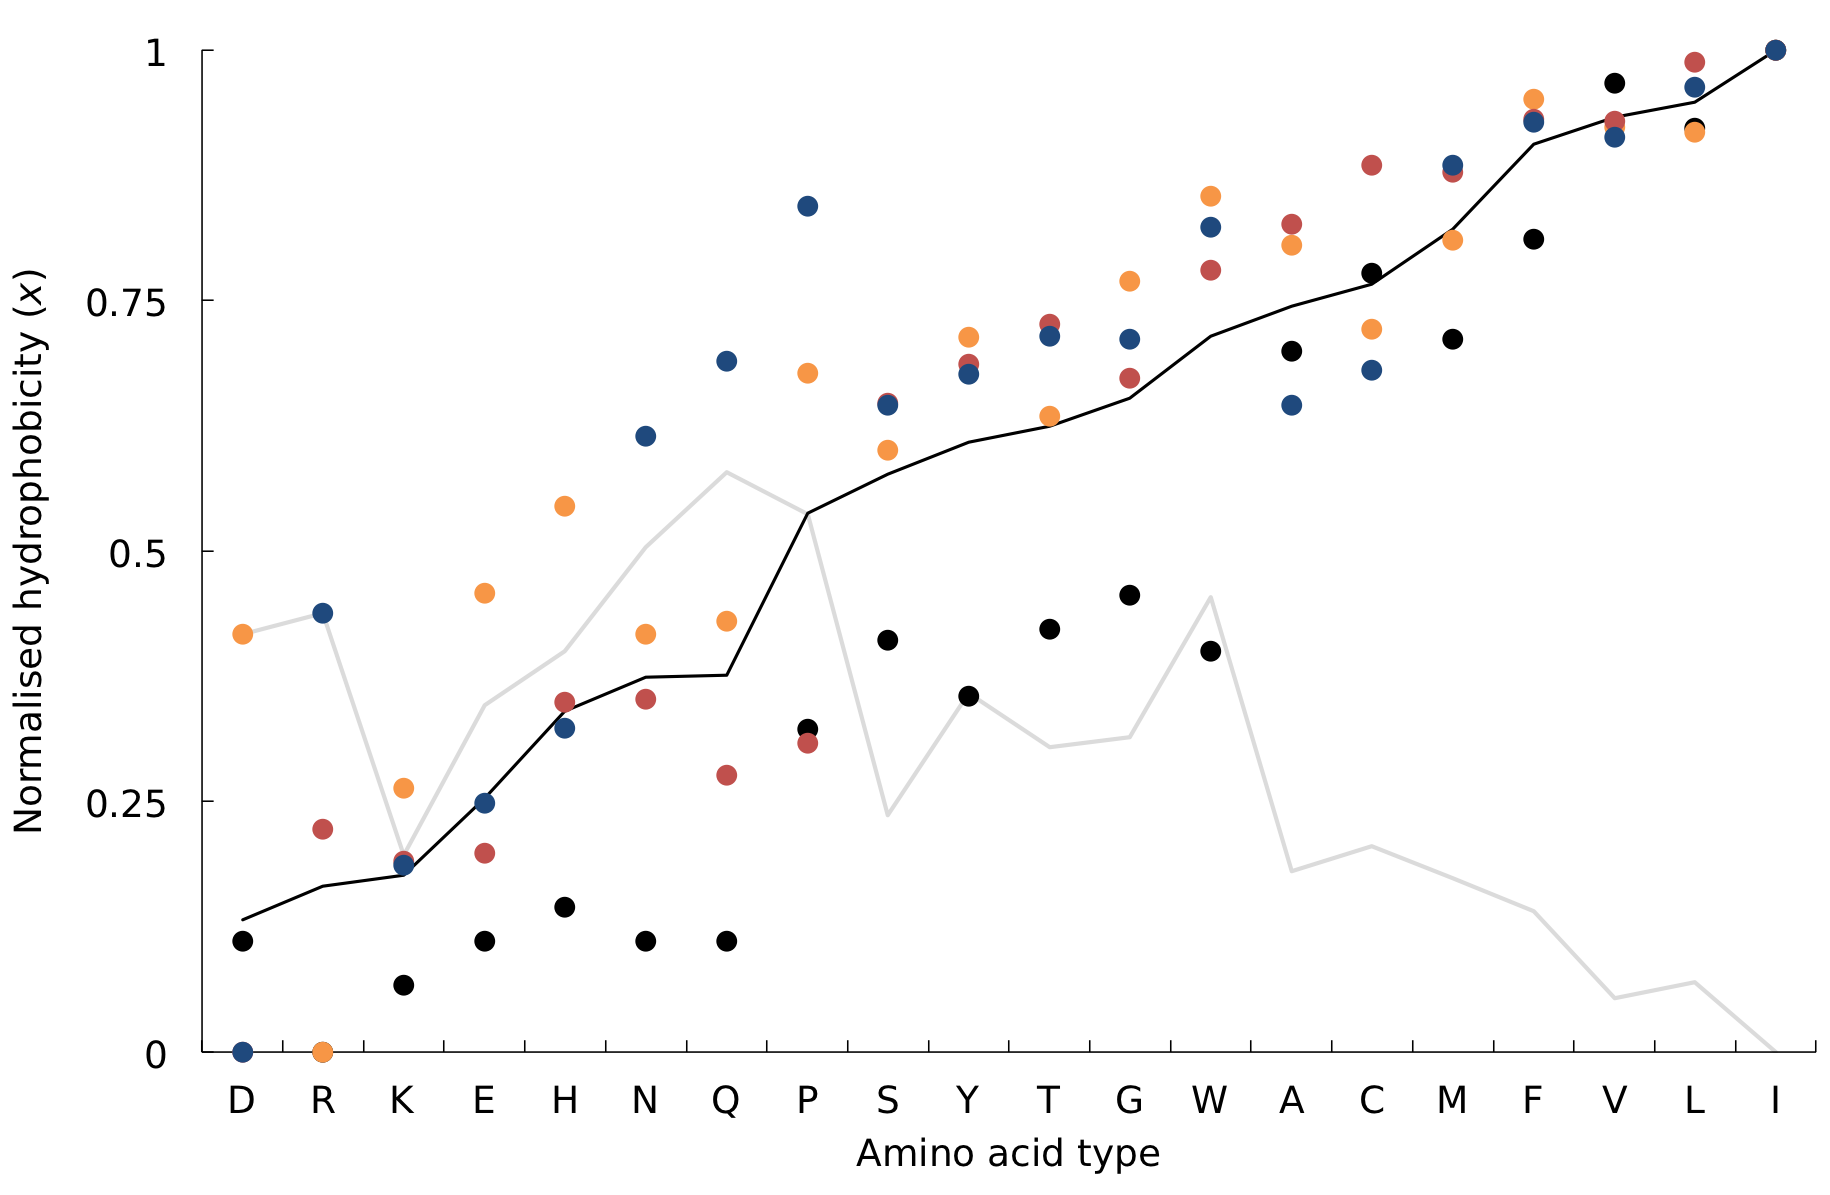
\includegraphics[width=1\textwidth]{Hydrophobicities}
\caption{A scatter plot comparing normalized values ($x$) of different hydrophobicity scales. Amino acids on the horizontal axis are arranged according to ${\bar{x}}_{r}$ taking into account all 4 scales. The points in blue are the White and Wimley scale~\cite{White1999}, in red is Hessa's biological scale~\cite{Hessa2005}, in orange is the Eisenberg consensus scale~\cite{Eisenberg1984}, and in black are the Kyte \& Doolittle values~\cite{Kyte1982}. The black line connects ${\bar{x}}_{r}$ values, whilst the gray line connects $|\underset{x_r}{\max}-\underset{x_r}{\min}|$, although obviously in both cases the line is only for illustrative purposes and does not show a relationship between the residues.}
\label{fig:normalisedhydrophobicity1}
\end{figure}
